\section{Besonderheiten von Vektoruhren}

Nach Betrachtung der Funktionsweise von Vektoruhren sowie einer Beschreibung von besonderen Problemen, gibt es noch weiterführende Aspekte zu beachten. Diese sind oberhalb einer reinen Betrachtung der Funktion von Vektoruhren angesiedelt und behandeln eher Themen wie die zeitliche Sortierung von Nachrichten oder eine Anbindung an eine Anwendungs-API, welche anhand der Informationen, welche Sie durch das darunterliegende Vektoruhr-System erhält, entscheidungen für den Programmablauf trifft. In diesem Kapitel wird der sogenannte Causally Ordered Multicast zum Ordnen von Nachrichten behandelt sowie auf die Rolle der Anwendungs-API innerhalb einer verteilten Systems mit Vektoruhren als Synchronisationsbasis eingegangen.
\subsection{Causaly Ordered Multicast}

In einem Verteilten System kann es recht schnell passieren, dass sich die Reihenfolge von gesendeten Broadcasts bei dem Empfänger und dem Sender unterscheiden. Dies führt in gewissen Fällen zu Problemen, wenn z.B. die Daten eines zweiten Broadcast von denen des ersten abhängen, es also eine temporale korrelation gibt. Um diesen Problem zu lösen, haben Kenneth P. Birman und Thomas A. Joseph in \cite{Birman:1987:RCP:7351.7478} den sogenannten Causal Brooadcast eingeführt, welcher auch als Causaly Ordered Multicast bezeichnet werden kann.

Wie in \cite{Birman:1987:RCP:7351.7478}[S. 52, Kapitel 3.3] beschrieben, kann es vorkommen, dass sich die Reihenfolge der gesendeten Nachrichten eines Senders und die Reihenfolge der empfangenen Nachrichten am Empfänger unterscheiden. Dies kann etwa durch Verzögerungen auf dem Übertragungsweg geschehen. Bei einem herkömmlichen Broadcast, welcher in einem System mit Vektoruhren abgesendet wird, ist kein Mechanismus vorgesehen, um eine eventuell für die Funktionsweise der Anwendung notwendige Reihenfolge der versendeten Nachrichten einzuhalten. Die Broadcast-Nachricht wird einfach an alle Teilnehmer versendet und nicht weiter beachtet.

Anders ist dies bei einem Causaly Orderen Multicast. Wie der Name bereit vermuten lässt, spielt hierbei die Ordnung der Multicasts nach deren Kausalität, also der Ursache eine Rolle. Die Ursache ist in diesem Fall das Verschicken des Broadcast am Sender. Somit werden bei einem Causal Broadcast die Nachrichten nach deren Reihenfolge des Versendens am Empfängerprozess geordnet. Um eine Rückantwort eines jeden Nodes an den Sender mit einer Empfangsbestätigung zu vermeiden, kann ein Causally Ordered Multicast auf Basis der Vektoruhren in den Empfängern umgesetzt werden. Durch die Vektoruhr kann ein Node entscheiden, ob er bei Empfang einer Nachricht alle Broadcast des entsprechenden Senders erhalten hat, die in der kausalen Vergangenheit dieses Broadcasts empfangen hat. Ist dies nicht der Fall, muss er die Nachricht in eine Warteliste setzten und diese erst annehmen, sobald alle in der Zwischenzeit passierten Broadcasts angekommen sind. Abbildung \ref{figure:causalbroadcast} verdeutlicht diese Funktionsweise genauer.

\begin{figure}[ht]
	\centering
	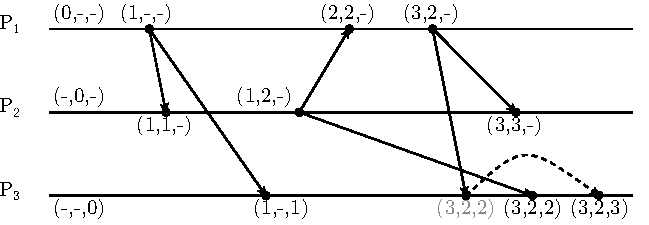
\includegraphics[width=10cm]{kommBeispielCausalBroadcast.pdf}
	\caption[Kommunikation durch Causally Ordered Multicasts]{Ablauf einer Kommunikation zwischen Prozessen, die ausschließlich Causally Ordered Multicasts versenden. Wie man sieht, muss ein Prozess eine Empfangene Nachricht aufheben, bis eine vorher gesendete Nachricht eintrifft.}
	\label{figure:causalbroadcast}
\end{figure}
\FloatBarrier

Der Ablauf des Aufhebens und Verzögerns von gewissen Nachrichten lässt sich durch ein recht einfaches Protokoll darstellen. Dieses ist in Abbildung \ref{figure:causalBroadcastProtocol} dargestellt.

\begin{figure}[ht]
	\centering
	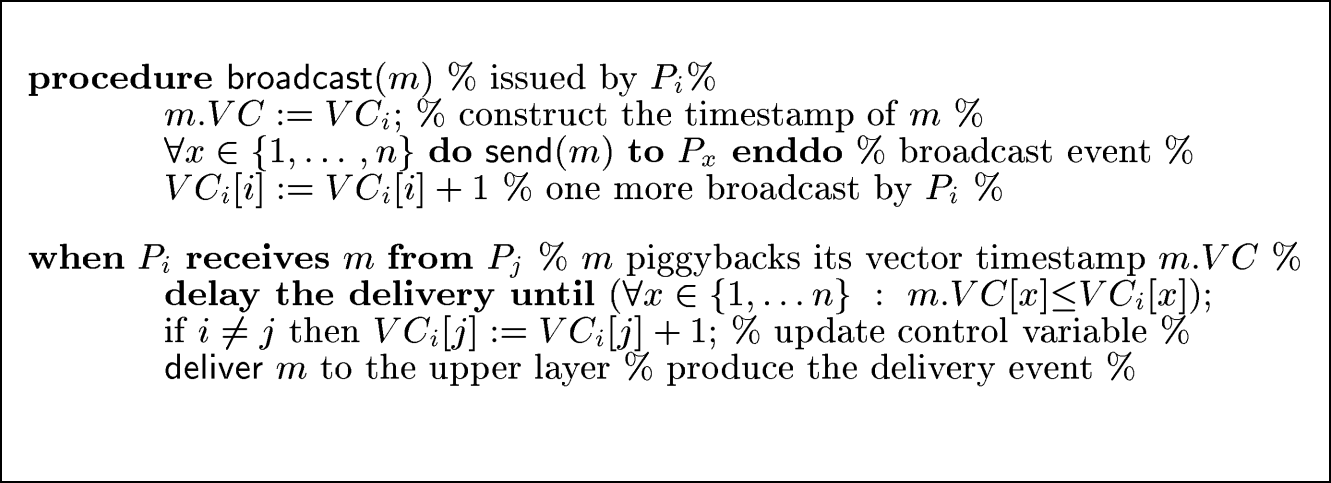
\includegraphics[width=10cm]{causalBroadcastProtocol.png}
	\caption[Protokoll für den Causally Ordered Multicast]{Beschreibung der verarbeitung von Causally Ordered Multicast in Form eines Protokolls.}
	Quelle: \cite{Baldoni:2002:FDC:1435723.1437765}[S. 7, Abbildung 3]
	\label{figure:causalBroadcastProtocol}
\end{figure}
\FloatBarrier

Ausgeschrieben sieht die Funktionalität des Protokolls folgendermaßen aus:

\begin{itemize}
	\item Löst ein Prozess durch ein stattgefundenes Event einen Broadcast aus, so fügt er zunächst seine aktuelle Vektoruhr an die Nachricht des Broadcasts an. Nun sendet er die Nachricht an alle teilnehmenden Prozesse und aktualisiert im letzten Schritt seinen Eintrag in der lokalen Vektoruhr.
	\item Empfängt ein Prozess $P_i$ eine Nachricht m des Prozesses $P_j$, so muss er die Nachricht so lange verzögern, bis die Bedingung $m.VC[x] \le VC_i[x]$ erfüllt ist, also bis die Nachricht ein direkter Nachfolger der Vorherigen ist. Anschließend wird der wert VC[j] inkrementiert, um das Sendeevent des Prozesses $P_j$ zu verzeichnen. Nun kann die Nachricht an die Anwendungsschicht weitergegeben werden.
\end{itemize}

Im Laufe der Kommunikation kann es passieren, dass mehrere nacheinander empfangenen Nachrichten nicht sofort verwendet sondern verzögert werden müssen. Für diesen Fall bietet es sich an, die verzögerten Nachrichten in einer liste zu speichern und bei Eintreffen einer neuen Nachricht alle zunächst zurückgehaltenen nach deren \qq{alter} sortiert zu verarbeiten.

Zu erwähnen ist an dieser Stelle, dass sich die Aktualisierung einer Vektoruhr wie in dem Protokoll beschrieben etwas von der urpsrünglichen, rein auf Vektoruhren ausgelegten Vorgehensweise unterscheidet. Wie Kapitel \ref{prinzipFunktion} unter Satz R1 bis R3 angegeben, inkrementiert ein Node seinen eigenen Eintrag in der lokalen Uhr bei auslösen eines jeden Events. Für Causally Ordered Broadcasts ist dies nur beim verschicken einer Nachricht der Fall, außerdem geschieht dies erst nach dem abschicken. Der Empfänger $P_i$ hat dann die Aufgabe, seine lokale Vektoruhr an der Stelle $VC_i[j]$ zu erhöhen, er ändert bei Causally Ordered Multicasts also den Eintrag eines anderen Prozesses in seiner lokalen Uhr anstatt wie vorher seinen eigenen. Durch diese Anpassung kennt jeder Prozess zu jeder Zeit die Anzahl an abgeschickten Broadcasts an allen Prozessen und kann bei Empfang einer Nachricht sehen, ob alle vorhergehend benötigten Broadcasts bereits eingetroffen sind.

\subsubsection{Umsetzung in C\# auf Basis der Vektoruhr}
Causaly Ordered Multicasts wurden als Erweiterung der in Kapitel \ref{vectorClockImpl} beschriebenen Implementierung eingefügt. In dem gewählten Bank-Szenario sendet ein Bankautomat bei jeder Kontoaktualisierung, also einem Event, einen Broadcast an alle im System vorhandenen Prozesse. Dabei ist es jedoch egal ob die gesendeten Nachrichten über die Aktualisierung auch ankommen oder nicht beziehungsweise spielt die Reihenfolge des Empfangs für den Sender keine Rolle. Dieses System funktioniert solange, bis ein Prozess einmal eine Aktualisierung zu spät erhält und somit seinen Kontostand nicht entsprechend zum richtigen Zeitpunkt aktualisiert. Um diesem Problem entgegenzuwirken, können Causal Broadcasts verwendet werden.

Als Grundlage dient die in Kapitel \ref{vectorClockImpl} implementierte Vektoruhren-Mechanik. Neben den im vorherigen Abschnitt erwähnten Anpassungen für die Art und Weise, wie lokale Vektoruhren inkrementiert werden, muss für die Umsetzung des Causal Broadcasts ein Speicher für Verzögerte Nachrichten eingeführt werden. Dies wurde in Form einer einfachen Liste gemacht, welche den Typ \code{Message} als Typparemeter hat.  

TODO: Sortieren der Liste etc.

Damit ankommenden Nachrichten eventuell aufgehoben werden können, muss die Methode \code{HandleCommunicationMessage()} angepasst werden. Diese akzeptiert in der einfachen Vektoruhr-Implementierung alle Nachrichten und verarbeitet deren Inhalt. In der erweiterten Umsetzung, \code{HandleCommunicationMessageOrdered() genannt,} findet vorher eine Überprüfung statt, ob die neue Nachricht akzeptiert wird oder verzögert werden muss. Als Bedingung wird hier geprüft, ob die zu prüfenden Uhr zeitlich gesehen kleiner als die aktuelle lokale Uhr ist. Solange dies der Fall ist, muss die Nachricht aufgeschoben werden. 
TODO: Aufheben von nicht akzeptierten Nachrichten am Code zeigen
 
\subsection{Rolle der Anwendungsschicht (Anwendungs-API)}
TODO
\label{RolleDerAnwendung}